\documentclass[12pt]{article}
\usepackage{amsmath}
\usepackage{amssymb}
\usepackage{geometry}
\usepackage{enumerate}
\usepackage{natbib}
\usepackage{float}%稳定图片位置
\usepackage{graphicx}%画图
\usepackage[english]{babel}
\usepackage{a4wide}
\usepackage{indentfirst}%缩进
\usepackage{enumerate}%加序号
\usepackage{multirow}%合并行
\usepackage{graphicx}
\usepackage{enumerate}
\usepackage{booktabs}
\usepackage{geometry}
\usepackage{indentfirst}
\usepackage{mathrsfs}
\usepackage[T1]{fontenc}
\usepackage{mathtools}
\usepackage{amsthm}
\usepackage{babel}
\usepackage{listings}
\usepackage{subfigure}
\usepackage{caption}
\usepackage{pgfplots}
\usepackage{wrapfig}
\usepackage{rotating}
\usepackage[section]{placeins}
\usepackage{subfigure}
\usepackage{textcomp}
\usepackage[normalem]{ulem}
\usepackage{tabularx}
\usepackage{color}
\usepackage{mathrsfs}
\usepackage{setspace}
\usepackage[colorlinks,linkcolor=blue]{hyperref}%超链接
\title{\large UM-SJTU JOINT INSTITUTE\\PROBABILISTIC  METHODS IN
ENGINEERING\\(VE401)\\\ \\\ \\\ \\\ \\\ \\\ \\\ \\\
PROJECT 1 REPORT\\\ \\\ TEAM PROJECT GROUP 30 \\\ \\\ \\\ \\\ \\\ }
\author{Authors' Name and ID\\Chen Zhibo \\Pan Chongdan 516370910121\\Shen Yuan \\Xiang Zhiyuan 516370910126\\Zhan Yan}
\date{Date: \today}

\begin{document}
\maketitle
\newpage
\section{Project Introduction}
Natural numbers, like physical constants, appear to have a non-uniform distribution of digits. Intuitively, we may consider that the leading digit of these numbers should have a uniform distribution. For example, the frequency of the numbers beginning with 1 should be approximately equal to the frequency of the numbers beginning with 9. However, it's clear that more numbers  begin with 1 in our real life than others. For instance, the height of any person measured in cm will most often begin with the
digit 1. Even if we change the unit, this mysterious phenomenon still happens.
\par Usually, when we first meet the distribution of frequency of digital in natural numbers, we think that data of uniform distribution is independent of re-scaling because every digital should play the some role. \\\
\par However, in \textbf{problem 1}, we show that if the leading digits of a discrete random variable follow a discrete uniform distribution (each digit occurs with probability 1/9) then this distribution is not independent of re-scaling.
\par If the leading digits of a discrete random variable follow a discrete uniform distribution, then this distribution is not a uniform distribution after multiplying 5. Denote the original random variable as X and after multiplying as Y. Then P[X=n]=1/9, n=1,2,...,9.
\begin{equation}
        \left.
        \begin{tabular}{cc}
            Leading digits & Possible leading digits after multiplying 5\\
            \hline
            1 & 5,6,7,8,9\\
            2,3 & 1\\
            4,5 & 2\\
            6,7 & 3\\
            8,9 & 4\\
        \end{tabular}
        \right.
        \end{equation}
        
Then we can see that P[Y=1]=P[Y=2]=P[Y=3]=P[Y=4]=2/9, while P[Y=5,6,7,8,9]=1/9 and this is not a uniform distribution.
\\\
\par Frank Benford independently noticed this effect in a book of logarithm tables where the
initial pages were much more worn by use than the later pages. He was the first to systematically investigate the
effect in 1938. The observed distribution of digits is now known as \emph{Benford’s law} or \emph{Benford’s distribution}. 
\par In our project, we focus on the occurrence of numbers in real life and study the following basic argument:
\par \textbf{Given a collection of naturally occurring numbers whose size is not constrained by outside effects,
the distribution of the leading digits should not depend on the units of measurement used.}
\section{Example in Reality}
\par For example, if the numbers are length measurements, the proportion of 1s, 2s, 3s, etc. should be the same,
whether the lengths are measured in meters, in feet or in any other unit system. Of course, individual lengths
will have different numerical expressions, but the overall distribution of leading digits should not be affected by
unit choice. This is a \textbf{scaling argument}, since it claims that the distribution of digits should be invariant under
re-scaling.

\par In \textbf{problem 2 and problem 3} we take a table of material constants, list the values of the
shear modulus for the solid elements. Create a histogram of their frequencies and comment on the data. Then we transform the data into another unit and get the tables and histogram again
\begin{table}[H]
\centering
\caption{Shear modulus for solid elements (The unit is E/GPa)}
\begin{tabular}{|c|c|c|c|c|c|c|c|c|}
\hline
Li & 4.2  & 4  & Nb & 38    & 3 & Dy & 24.7 & 2 \\ \hline
Be & 132  & 1  & Mo & 120   & 1 & Ho & 26.3 & 2 \\ \hline
Na & 3.3  & 3  & Ru & 173   & 1 & Er & 28.3 & 2 \\ \hline
Mg & 17   & 1  & Rh & 150   & 1 & Tm & 30.5 & 3 \\ \hline
Al & 26   & 2  & Pd & 44    & 4 & Yb & 9.9  & 9 \\ \hline
K  & 1.3  & 1  & Ag & 30    & 3 & Lu & 27.2 & 2 \\ \hline
Ca & 7.4  & 7  & Cd & 19    & 1 & Hf & 30   & 3 \\ \hline
Sc & 29.1 & 2  & Sn & 18    & 1 & Ta & 69   & 6 \\ \hline
Ti & 44   & 44 & Sb & 20    & 2 & W  & 161  & 1 \\ \hline
V  & 47   & 4  & Te & 16    & 1 & Re & 178  & 1 \\ \hline
Cr & 115  & 1  & Ba & 4.9   & 4 & Os & 222  & 2 \\ \hline
Fe & 82   & 8  & La & 14.3  & 1 & Ir & 210  & 2 \\ \hline
Co & 75   & 7  & Ce & 13.5  & 1 & Pt & 61   & 6 \\ \hline
Ni & 76   & 7  & Pr & 14.8  & 1 & Au & 27   & 2 \\ \hline
Cu & 48   & 4  & Nd & 16..3 & 1 & Tl & 2.8  & 2 \\ \hline
Zn & 43   & 4  & Pm & 18    & 1 & Pb & 5.6  & 5 \\ \hline
Se & 3.7  & 3  & Sm & 19.5  & 1 & Bi & 12   & 1 \\ \hline
Sr & 6.1  & 6  & Eu & 7     & 2 & Th & 31   & 3 \\ \hline
Y  & 25.6 & 2  & Gd & 22    & 2 & U  & 111  & 1 \\ \hline
Zr & 33   & 3  & Tb & 22.1  & 2 & Pu & 43   & 4 \\ \hline
\end{tabular}
\end{table}
\begin{figure}[H]
\centering
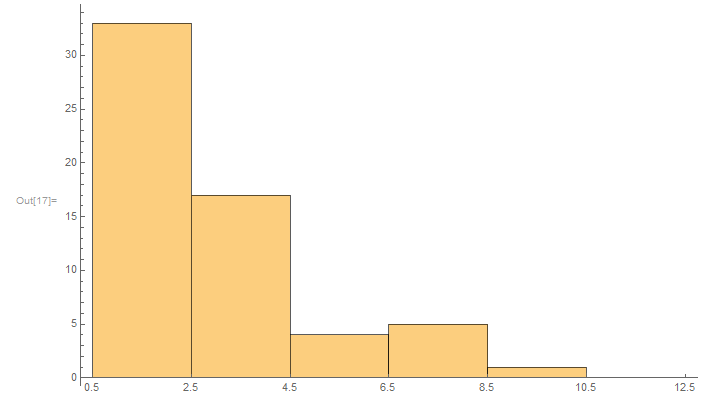
\includegraphics[scale=0.38]{P1.png}
\caption{The corresponding histogram}
\end{figure}
The first histogram is the frequency of the first digit of the sheer modulus of different elements in $N/m^2$. From the histogram we can see that almost half of the numbers starting with 1 and quarter of the numbers starting with 2.
\par Then I change the unit from $E/GPa$ to $oz/tf^2$ and the following value table:
\begin{table}[H]
\centering
\caption{Shear modulus for solid elements (The unit is E/GPa)}
\begin{tabular}{|c|c|c|c|c|c|c|c|c|}
\hline
Li & 13  & 1 & Nb & 124 & 1 & Dy & 80  & 8 \\ \hline
Be & 435 & 4 & Mo & 393 & 3 & Ho & 86  & 8 \\ \hline
Na & 10  & 1 & Ru & 567 & 5 & Er & 92  & 9 \\ \hline
Mg & 55  & 5 & Rh & 491 & 4 & Tm & 99  & 9 \\ \hline
Al & 85  & 8 & Pd & 144 & 1 & Yb & 32  & 3 \\ \hline
K  & 4   & 4 & Ag & 98  & 9 & Lu & 89  & 8 \\ \hline
Ca & 24  & 2 & Cd & 62  & 6 & Hf & 98  & 9 \\ \hline
Sc & 95  & 9 & Sn & 59  & 5 & Ta & 226 & 2 \\ \hline
Ti & 144 & 1 & Sb & 65  & 6 & W  & 527 & 5 \\ \hline
V  & 154 & 1 & Te & 52  & 5 & Re & 583 & 5 \\ \hline
Cr & 377 & 3 & Ba & 16  & 1 & Os & 727 & 7 \\ \hline
Fe & 268 & 2 & La & 46  & 4 & Ir & 688 & 6 \\ \hline
Co & 245 & 2 & Ce & 44  & 4 & Pt & 199 & 1 \\ \hline
Ni & 249 & 2 & Pr & 48  & 4 & Au & 88  & 8 \\ \hline
Cu & 157 & 1 & Nd & 53  & 5 & Tl & 9   & 9 \\ \hline
Zn & 140 & 1 & Pm & 59  & 5 & Pb & 18  & 1 \\ \hline
Se & 12  & 1 & Sm & 63  & 6 & Bi & 39  & 3 \\ \hline
Sr & 19  & 1 & Eu & 25  & 2 & Th & 101 & 1 \\ \hline
Y  & 83  & 8 & Gd & 71  & 7 & U  & 363 & 3 \\ \hline
Zr & 108 & 1 & Tb & 72  & 7 & Pu & 140 & 1 \\ \hline
\end{tabular}
\end{table}
\begin{figure}[H]
\centering
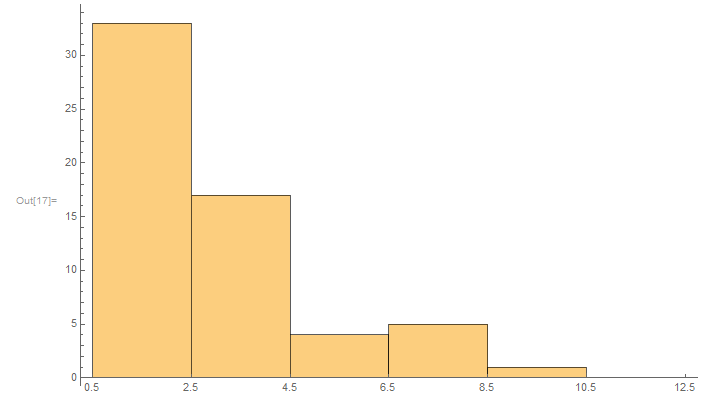
\includegraphics[scale=0.4]{P1.png}
\caption{The corresponding histogram}
\end{figure}
From the two histograms we can see most data start with digital 1 and the distribution of other numbers doesn't depend much on the choice of the units.

\section{Benford Law}
Since we already have a rough idea about the definition of Benford Law and Benford distribution, now let's study Benford Law more deeply and find its formula.
\subsection{Pinkham's Proof}
\par One convincing argument as to why Benford’s law should hold is that the occurrence of digits should
follow a distribution that does not change when units are changed and the data is rescaled. Pinkham
gave an argument that purported to show that this scale invariance implies Benford’s law. In \textbf{Poblem 4}, we restate Pinkham's proof by ourself.
\par
So first let's think about one question, why would Pinkham thought the distribution should have the form $log_{10}(n+1)$?
\par Suppose one has a horizontal circular disc of unit circumference which is pivoted at the center. Let the disc be given a random angular displacement $\theta$ where $-\infty <\theta<\infty$. We can define the final position of the disc mod one is $\varphi$.
\begin{equation*}
\varphi \equiv \theta mod(1),\hspace{1cm}0\leq\varphi<1,
\end{equation*}
\par If we then define
\begin{equation*}
Pr(x\leq\theta<x+dx)=g(x)dx,
\end{equation*}
and
\begin{equation*}
Pr(y\leq\varphi<y+dy)=f(y)dy,
\end{equation*}
Because, assume $G(x)$ and $F(y)$ are the cumulative density function of variable $X,Y$, then we can get
\begin{equation*}
Pr(x\leq\theta<x+dx)=G(x+dx)-G(x);
Pr(y\leq\varphi<y+dy)=F(y+dy)-F(y);
\end{equation*}
\par So that as $dx\rightarrow 0$ and $dy\rightarrow 0$, $\dfrac{G(x+dx)-G(x)}{dx}=g(x)$
\par and $\dfrac{F(y+dy)-F(y)}{dy}=f(y)$.
\par And we know $\varphi \equiv \theta mod(1)$, and $f(y)$ equals to the probability density function of $\varphi$ at y, $g(x)$ equals to the probability density function of $\theta$ at x, so that
\begin{equation*}
f(y)=\sum\limits_{m=-\infty}^\infty g(y+m).
\end{equation*}
\par It is obvious that for a wide range of possible distributions of $\theta$ the distribution of $\varphi$ should be approximately uniform, that is
\begin{equation*}
 f(y)\approx1,\hspace{1cm} 0\leq y\leq 1,
\end{equation*}
\par This and related properties of distribution wrapped around a circle have been proved in Dvoretsky [].
\par Actually, the logarithmic law of left-most significant digits is a consequence of the above property of random variables mod one. Now let me show you.
\par Let $F(x)$ be the cumulative distribution function for the population of physical constants (taken non-negative for convenience). Define $D(x)$ by
\begin{equation*}
D(x)=\sum\limits_{m=-\infty}^\infty [F(x10^m)-F(10^m)], \hspace{1cm} x>0,
\end{equation*}
\par $D(n)$ for $n=2,3,...10$ gives the proportion of the population with first significant digit $n-1$ or less. The logarithmic "law" states that $D(n)$ should be approximately $log_{10}(n)$. Thus we suspects that
\begin{equation*}
log_{10}(x)\approx \sum\limits_{m=-\infty}^\infty [F(x10^m)-F(10^m)].
\end{equation*}
\par Then we change it into another form. Let define y as
\begin{equation*}
y=log_{10}(x)\hspace{0.4cm} and \hspace{0.4cm} G(y)=F(10^y).
\end{equation*}
\par Then we have
\begin{equation*}
y\approx \sum\limits_{m=-\infty}^\infty [G(y+m)-G(m)],
\end{equation*}
\par then we take derivatives, we can get
\begin{equation*}
1\approx \sum\limits_{m=-\infty}^\infty g(y+m).
\end{equation*}
\par So it's reasonable for Pinkham to consider $log_{10}(n+1)$ as the correct answer. And now we'll show you exactly how Pinkham proved his hypothesis.





\par 
Consider the population of all physical constants and the derived distribution of first significant digits. Suppose all the physical constants were multiplied by some fixed number. What would happen to the distribution of first significant digits? One may guess it would be the same as before. This invariance property has given us a method to characterize the distribution.
Now let's suppose $F(x)$ is the cumulative distribution for the population of all physical constants (assumed non-negative) in accordance with their size. Then let's define:
\begin{equation*}
(1)\hspace{2cm}D(x)=\sum\limits_{m=-\infty}^\infty [F(x10^m)-F(10^m)],\hspace{1cm}x>0
\end{equation*}
\par Obviously $D(n)$ for $n=2,3......9,10$ gives the proportion with first significant digit $n-1$ or less, because $F(x10^m)-F(10^m)$ represent the proportion with first significant digit $n-1$ or less in the range $(10^{m},10^{m+1}]$.
Assume $D(x)$ won't change when all the physical constants are multiplied by a positive constant $c$, then the resulting cumulative is $F(x/c)$, then we can get:
\begin{equation*}
(i)\hspace{2cm}D(x)=\sum\limits_{n=-\infty}^\infty [F(\dfrac{x}{c}10^m)-F(\dfrac{10^m}{c})]
\end{equation*}
And that equals to:
\begin{equation*}
(2)\hspace{2cm}D(n)=D(\dfrac{n}{c})-D(\dfrac{1}{c}),\hspace{1cm}c>0;n=2,...,10.
\end{equation*}
\par Actually, we only need the case $c=2$ or $10$, then we can prove $D(x)=log_{10}(x), x>0$.\\
To get this, we need to prove a theorem first:\\
\par {\textbf{Theorem 1}} If\\
$1. \hspace{3cm} D(2)+D(x)=D(2x),\hspace{3cm} x>0;$\\
$2. \hspace{2.56cm} D(10)+D(x)=D(10x),\hspace{3cm} x>0;$\\
$3. \hspace{3.5cm} D(x) is continous;$\\
$4. \hspace{4cm} D(10)=1;$\\
Then $D(x)=log_{10}(x), x>0.$\\
\par To prove this theorem, first, let's define $H(x)=D(10^x)$. Then we can find that conditions 1 and 2 becomes
\begin{equation*}
(3)\hspace{2cm} H(logn)+H(y)=H(logn+y),\hspace{1cm} -\infty <y< \infty, n=2,10.
\end{equation*}
\par For any $n=2$ or $10$, if we let $y=logn$, then we can get that $H(logn)+H(logn)=H(2logn)=2H(logn)$, then let's continue adding $H(logn)$ for $N$ times, then we can get:\\
$NH(logn)=H(Nlogn)$.\\
And if we let $n=10$, since $D(10)=1$, so that $H(log10)=H(1)=D(10)=1$, so that:\\
$H(N)=NH(log10)=N$.\\
\par Now, before I continue my proof, let me first introduce $Continued\;Fractions$ to you.\\
We define the function \\
\begin{center}
$a_0+\dfrac{1}{a_1+\dfrac{1}{a_2+\dfrac{1}{a_3+...+\dfrac{1}{a_N}}}}$\\
\end{center}
of the $N+1$ variables $a_0,a_1,a_2,...,a_n,...,a_N$ as a $finite\;continued\;fraction$. And if $a_0,a_1,....a_N\in N^*$, then we call it $Simple\;continued\;fraction$, and my proof only concern about $Simple\;continued\;fraction$. And we can also express this function in a different way:
\begin{center}
$[a_0,a_1,...,a_N]$.\\
\end{center}
So it's easy for us to find that:
\begin{equation*}
(4)\hspace{2cm}[a_0,a_1,...,a_N]=[a_0,a_1,...,a_{N-1}+\dfrac{1}{a_N}]
\end{equation*}
\par And we call $[a_0,a_1,...,a_n]$ with $n\leq N$ the $n$th convergent to $[a_0,a_1,...,a_N]$.
and then we define $p_n$ and $q_n$ as follows:\\
$p_0=a_0, p_1=a_1a_0+1, p_n=a_np_{n-1}+p_{n-2} (2\leq n\leq N),$\\
$q_0=1,q_1=a_1, q_n=a_nq_{n-1}+q_{n-2} (2\leq n\leq N),$\\
\par Obviously for any $n\in N$, $p_n\geq1,q_n\geq1$, then we can get
\begin{equation*}
(5)\hspace{2cm}[a_0,a_1,...,a_n]=\dfrac{p_n}{q_n}
\end{equation*}
by mathematical induction:\\
\par The definition of $p_n,q_n$ has already verify the case for $n=0$ and $n=1$. Now let's suppose it to be true for $1\leq m< N$.\\
\par That means $[a_0,a_1,...,a_{m-1},a_m]=\dfrac{p_m}{q_m}=\dfrac{a_mp_{m-1}+p_{m-2}}{a_mq_{m-1}+q_{m-2}}$,\\
\par Since the value of $p_{m-1},p_{m-2},q_{m-1},q_{m-2}$ depend only on $a_0,a_1,...,a_{m-1}$.\\
\par Hence using equation (4) we can get:
\begin{center}
$[a_0,a_1,...,a_m,a_{m+1}]=[a_0,a_1,...,a_{m-1},a_m+\dfrac{1}{a_{m+1}}]$\\
$=\dfrac{(a_m+\dfrac{1}{a_{m+1}})p_{m-1}+p_{m-2}}{(a_m+\dfrac{1}{a_{m+1}})q_{m-1}+q_{m-2}}$\\
$=\dfrac{a_{m+1}(a_mp_{m-1}+p_{m-2})+p_{m-1}}{a_{m+1}(a_mq_{m-1}+q_{m-2})+q_{m-1}}$\\
$=\dfrac{a_{m+1}p_m+p_{m-1}}{a_{m+1}q_m+q_{m-1}}=\dfrac{p_{m+1}}{q_{m+1}};$\\
\end{center}
So by mathematical induction we know (5) is right.

\par And $p_nq_{n-1}-p_{n-1}q_n=-(p_{n-1}q_{n-2}-p_{n-2}q_{n-1})$, and by mathematical induction we can continue this kind of calculation, and finally we can get:
\begin{equation*}
(6)\hspace{2cm}p_nq_{n-1}-p_{n-1}q_n=(-1)^{n-1}.
\end{equation*}
\par And in the same way, we can get:
\begin{equation*}
(7)\hspace{2cm}p_nq_{n-2}-p_{n-2}q_n=(-1)^na_n.
\end{equation*}
\par Now let's only consider that $a_1>0,...,a_N>0$, and they are integers, and for $n\in N$, let $x_n=\dfrac{p_n}{q_n}$.
\par Firstly, every $q_n$ is positive, so that, according to (6) (7), for $n\geq2$,\\ $x_n-x_{n-2}=\dfrac{p_nq_{n-2}-p_{n-2}q_n}{q_nq_{n-2}}=(-1)^n\dfrac{a_n}{q_nq_{n-2}}$ has the sign of $(-1)^n$, we can get:\\

\par {\textbf{Theorem 2}}: For $n\in N$, the even convergence $x_{2n}$ increase strictly with $n$, while the odd convergence $x_{2n+1}$ decrease strictly.\\

And since for $n\geq 1$, $x_n-x_{n-1}=\dfrac{p_nq_{n-1}-p_{n-1}q_n}{q_nq_{n-1}}$ has the sign of $(-1)^{n-1}$, so that for $m\in N$, $(-1)^{2m}=1$, that means $x_{2m+1}>x_{2m}$.
Now we can use Theorem 2 to prove Theorem 3:\\

\par {\textbf{Theorem 3}}: Every odd convergent is greater than any even convergent.\\

We can prove it by contradiction. If the Theorem were false, for $m,u\in N$, we should have $x_{2m+1}\leq x_{2u}$ for some pair $m,u$. If $u<m$, then according to Theorem 2, $x_{2m+1}<x_{2m}$, and if $u>m$, then $x_{2u+1}<x_{2u}$, and either inequality contradicts, which means Theorem 3 is true.\\
\par Then we use mathematical induction to prove Theorem 4:\\

\par {\textbf{Theorem 4}}: $q_n\geq n$ with inequality when $n>3$.\\

First, because $q_0=1, q_1=a_1\geq 1$, that means Theorem 4 is true for $n<2$. And if $n\geq 2$, since $a_n\in N^*$ and for any $n\in N$, $p_n\geq1, q_n\geq1$, then

$q_n=a_nq_{n-1}+q_{n-2}\geq q_{n-1}+1$

so that $q_n>q_{n-1}$ and $q_n\geq n$. If $n>3$, then

$q_n\geq q_{n-1}+q_{n-2}>q_{n-1}+1\geq n$,

and so we have proved that Theorem 4 is true.\\
\par Now we can use the Theorems we have proved above to prove that:\\
\\
$\blacktriangleright${\textbf{For a infinite simple continued fraction that is $[a_0,a_1,...]$, with $a_1>0,...,a_n>0,...,$ then $[a_0,a_1,...]$ converge to a limit x.}}\\

First we can assume $x_n=\frac{p_n}{q_n}=[a_0,a_1,...,a_n]$ is the $n$th convergent of $[a_0,a_1,...,a_N]$, where $N\rightarrow \infty$, hence by theorem 2, the even convergence form an increasing and the odd convergence a decreasing sequence.

\par And by Theorem 3 we know that every even convergent is less than $x_1$, so that the increasing sequence of even convergence is bounded above, and every odd convergent is greater than $x_0$, so that the decreasing sequence of odd convergence is bounded below. Hence the even convergence tend to a limit $e_1$, while the odd convergence tend to a limit $e_2$, with $e_1\leq e_2$.

Finally according to (6) and Theorem 4 we can get:
\begin{equation*}
|\dfrac{p_{2n}}{q_{2n}}-\dfrac{p_{2n-1}}{q_{2n-1}}|=\dfrac{1}{q_{2n}q_{2n-1}}\leq\dfrac{1}{2n(2n-1)}\rightarrow0.
\end{equation*}
\par So that $e_1=e_2=x$, so it converges to $x$. So we get Theorem 5:\\
\par {\textbf{Theorem 5}}: For an infinite simple continued fraction that is $[a_0,a_1,...]$, with $a_1>0,...,a_n>0,...$, then $[a_0,a_1,...]$ converges to a limit $x$.\\
\par Now let's introduce $the\;continued\;fraction\;algorithm$.\\
\par Let $x$ be any real number, and let $a_0=[x]$, here $[x]$ means the largest integer that less than $x$. Then we can get:
\begin{equation*}
x=a_0+e_0, 0\leq e_0<1.
\end{equation*}
\par If $e_0\neq0,$ we can write:
\begin{equation*}
\dfrac{1}{e_0}=a'_1, [a'_1]=a_1, a'_1=a_1+e_1, 0\leq e_1<1.
\end{equation*}
\par If $e_1\neq 0$, we can write:
\begin{equation*}
\dfrac{1}{e_1}=a'_2=a_2+e_2, 0\leq e_2<1,
\end{equation*}
\par and so on. Also $a'_n=\dfrac{1}{e_{n-1}}>1$, and so $a_n\geq 1$, for $n\geq 1$. Thus
\begin{equation*}
x=[a_0,a'_1]=[a_0,a_1+\dfrac{1}{a'_2}]=[a_0,a_1,a'_2]=[a_0,a_1,a_2,a'_3]=...,
\end{equation*}
\par where $a_0,a_1,a_2,...$ are integers and
$a_1>0,a_2>0,...$\\
\par The system of equations:\\
\begin{center}
$x=a_0+e_0 (0\leq e_0<1),$\\
$\dfrac{1}{e_0}=a'_1=a_1+e_1 (0\leq e_1<1),$\\
$\dfrac{1}{e_1}=a'_2=a_2+e_2 (0\leq e_2<1),$\\
$...$
\end{center}
is known as the $continued\;fraction\;algorithm$. The algorithm continues so long as $e_n\neq0$.
\par So that means for any rational $x$, we can always find $N$ such that $x=[a_0,a_1,...,a_N]$.
\par And obviously, for an infinite simple continued fraction, it converges to an irrational fraction, if not, the algorithm would terminate at a specific $N$.\\

So now after proving all the Theorems above, we get a useful conclusion to help us solve the invariance principle, that is:

For $x=log2$, we can find an infinite continued fraction which converges to $x$. That means:\\
\begin{center}
$log2=(\dfrac{p_m}{q_m})+o(\dfrac{1}{p_m})\hspace{2cm}(m\rightarrow\infty)$
\end{center}
Thus, we have:
\begin{equation*}
q_m log2=p_m+o(1)\qquad(m\rightarrow \infty)
\end{equation*}
which indicates that 
\begin{equation*}
q_mH(log2)=H(q_mlog2)=H(p_m+o(1))=H(p_m)+H(o(1))=p_m+H(o(1))
\end{equation*}
\par According to hypothesis 2 and 4, we have:
\begin{equation*}
D(x)=D(10x)-1
\end{equation*}
\par Considering that $D(x)$ is continuous, we can know that
\begin{equation*}
\lim_{x\to1} D(x)=\lim_{x\to1}D(10x)-1=D(10)-1=0
\end{equation*}
which suggests that
\begin{equation*}
\lim_{x\to0}H(x)=\lim_{x\to0}D(10^x)=\lim_{x\to1}D(x)=0
\end{equation*}
\par Therefore, we can conclude that 
\begin{equation*}
q_mH(log2)=q_m+o(1)
\end{equation*}
\par By the fact that $q_m log2=p_m+o(1)$ and $q_mH(log2)=p_m+o(1)$ when $m$ approaches infinity, we have:
\begin{equation*}
H(log2)=log2
\end{equation*}
\par According to (3), $H(y+1)=H(y)+H(1)=H(y)+1, -\infty<y<\infty$, which suggests that $H(y+2)=H(y+1+1)=H(y+1)+1=H(y)+2$ and $H(y-1)=H(y-1+1)-H(1)=H(y)-1$. Assuming that for $t\in [-k,k], k\in \mathbb{N^*}, H(y+t)=H(y)+t$, we have:
\[
\begin{split}
H(y+k+1)=H(y+k)+1=H(y)+k+1 \\
H(y-k-1)=H(y-k)-1=H(y)-k-1
\end{split}
\]
\par Hence, by mathematical induction, we can know that $H(y+t)=H(y)+t, t\in \mathbb{Z}, y\in \mathbb{R}$.
\par Moreover, for $\forall y \in \mathbb{R}, y=[y]+y-[y]$ and $H(y)=H([y]+y-[y])=H([y])+H(y-[y])=[y]+H(y-[y])$. Due to the fact that $y-[y]\in [0,1)$, we only need to prove that for $\forall x \in [0,1), H(x)=x $\ to derive the conclusion that $H(x)=x$ (so $D(x)=log_{10}x$).
\par To prove the last part of our theory, we need to focus on the problem proved by H. Weyl in 1917 first.The problem is that for every irrational 
$\alpha$, the sequence $\alpha _n=n\alpha-[n\alpha], n\in \mathbb{N^*}$ is equidistributed in [0,1]. We will prove this conclusion step by step.
\par Firstly, we establish several notations we will use in the proof. Let $\omega=(x_n), n\in \mathbb{N^*}$ be a given sequence of real numbers. For a positive integer $N$ and a subset $E$ of $I=[0,1)$, let the counting function $A(E;N;\omega)$ be defined as the number of terms $x_n,1\le n\le N$, for which ${x_n}\in E$. Here is our basic definition of equidistribution.
\par {\textbf{Definition 1}} The sequence $\omega=(x_n), n\in \mathbb{N^*}$ of real numbers is said to be \emph{uniformly distributed modulo 1} if for every pair $a,b$ of real numbers with $0\le a<b\le 1$, we have:
\begin{equation*}
\lim_{N\to \infty}\frac{A([a,b);N;\omega)}{N}=b-a
\end{equation*}
\par {\textbf{ Definition 2}} Let X be a universal set and A be a subset of X. For $\forall x\in X$, we define the characteristic function of A as:

\begin{equation*}
c_A\{x\}=
\begin{cases}
1, &x\in A\\
0, &x\notin A
\end{cases}
\end{equation*}

\par Let $c_{[a,b)}$ be the characteristic function of the interval $[a,b)\subset I$.Then, the  definition 1 can be written in the integral form as follows:
\begin{equation*}
\lim_{N\to\infty}\frac{1}{N}\sum_{n=1}^{N}c_{[a.b)} (\{x_n\})=\int_{0}^{1}c_{[a,b)}(x)dx
\end{equation*}
where $\{x_n\}=x-[x]$ is the fractional part of $x$.
This observation with a significant approximation technique, can lead to the following criterion.
\par {\textbf{Theorem 6}} The sequence $(x_n), n\in \mathbb{N^*}$ of real numbers is uniformly distributed mod 1 if and only if for every real-valued continuous (or piecewise continuous)function $f$ defined on the closed unit interval $\bar{I}=[0,1]$, we have:
\begin{equation*}
\lim_{N\to\infty}\frac{1}{N}\sum_{n=1}^{N}f(\{x_n\})=\int_{0}^{1}f(x)dx
\end{equation*}
\par Proof: Let $(x_n)$ be uniformly distributed mod 1, and let $f(x)=\sum\limits_{i=0}^{k-1}d_ic_{[a_i,a_{i+1})}(x)$ be a step function on $\bar{I}$, where $0=a_0<a_1<\ldots<a_k=1$. According to the integral form of definition 1, for every such function $f$, we have:
\begin{equation*}
\lim_{N\to\infty}\frac{1}{N}\sum_{n=1}^{N}f(\{x_n\})=\int_{0}^{1}f(x)dx
\end{equation*}
\par We now assume that $f$ is a real-valued continous (or piecewise continous) function defined on $\bar{I}$, which is naturally Darboux-integrable by Vv186. For $\forall \epsilon >0$, by the definition of the Darboux integral, there exist two step functions $f_1$ and $f_2$ such that $f_1(x)\leq f(x)\leq f_2(x), \forall x \in \bar{I}$ and $\int_{0}^{1}(f_2(x)-f_1(x))dx\leq\epsilon$. In consequence, we have:
\[
\begin{split}
\int_{0}^{1}f(x)dx-\epsilon\leq\int_{0}^{1}f_1(x)dx=\lim_{N\to\infty}\frac{1}{N}\sum_{n=1}^{N}f_1(\{x_n\}) \\
\leq \varliminf_{N\to\infty}\frac{1}{N}\sum_{n=1}^{N}f(\{x_n\})\leq \varlimsup_{N\to \infty}\frac{1}{N}\sum_{n=1}^{N}f(\{x_n\}) \\
\leq \lim_{N\to \infty}\frac{1}{N}\sum_{n=1}^{N}f_2(\{x_n\})=\int_{0}^{1}f_2(x)dx\leq \int_{0}^{1}f(x)dx+\epsilon
\end{split}
\]
where we have use the definition that $\varliminf\limits_{N\to\infty} a_n$ and $\varlimsup\limits_{N\to\infty} a_n$ represent the limes superior and limes inferior for a bounded real sequence $(a_n)$ respectively and the conclusion that $\varliminf\limits_{N\to\infty} a_n \leq \varlimsup\limits_{N\to\infty} a_n$ by Assignment 3 in Vv186.
\par As $\epsilon$ can be arbitrarily small, we can know that 
\begin{equation*}
\varliminf_{N\to\infty}\frac{1}{N}\sum_{n=1}^{N}f(\{x_n\})= \varlimsup_{N\to \infty}\frac{1}{N}\sum_{n=1}^{N}f(\{x_n\}) =\int_{0}^{1}f(x)dx
\end{equation*}
\par Again, by Assignment 3 in Vv186, we can conclude that 
\begin{equation*}
\lim_{N\to\infty}\frac{1}{N}\sum_{n=1}^{N}f(\{x_n\})=\int_{0}^{1}f(x)dx
\end{equation*}
\par Now let's prove the sufficiency of Thoerem 6. Let a sequence $(x_n)$ be given and $[a,b)$ be an arbitrary subinterval of $I$. Considering that the characteristic function $c_{[a,b)}$ is actually a step function, for $\forall \epsilon >0$, there exist two piecewise continuous functions $g_1$ and $g_2$ such that $g_1(x)\leq c_{[a,b)}(x)\leq g_2(x), \forall x\in \bar{I}$ and $\int_{0}^{1}(g_2(x)-g_1(x))dx\leq\epsilon$. As a result, we have:
\[
\begin{split}
b-a-\epsilon\leq \int_{0}^{1}g_2(x)dx-\epsilon\leq \int_{0}^{1}g_1(x)dx=\lim_{N\to\infty}\frac{1}{N}\sum_{n=1}^{N}g_1({x_n})\\
\leq \varliminf_{N\to\infty}\frac{A([a,b);N;x)}{N}\leq \varlimsup_{N\to\infty}\frac{A([a,b);N;x)}{N}\leq \lim_{N\to\infty}\frac{1}{N}\sum_{n=1}^{N}g_2({x_n})\\
=\int_{0}^{1}g_2(x)dx\leq \int_{0}^{1}g_1(x)dx+\epsilon\leq b-a+\epsilon
\end{split}
\]
\par As $\epsilon$ can be arbitrarily small, we have:
\begin{equation*}
\varliminf_{N\to\infty}\frac{A([a,b);N;x)}{N}= \varlimsup_{N\to\infty}\frac{A([a,b);N;x)}{N}=b-a
\end{equation*}
which indicates that
\begin{equation*}
\lim_{N\to\infty}\frac{A([a,b);N;x)}{N}=b-a
\end{equation*}
\par By Definition 1, we can know that the sequence $(x_n)$ is uniformly distributed mod 1. 
\par \qed
\par By Thoerem 6, we can prove the following corollary.
\par {\textbf{Corollary}} The sequence $(x_n)$ is uniformly distributed mod 1 if and only if for every complex-valued continuous (or piecewise continuous) function $f$ on $\mathbb{R}$ with period 1 we have:
\begin{equation*}
\lim_{N\to\infty}\frac{1}{N}\sum_{n=1}^{N}f(x_n)=\int_{0}^{1}f(x)dx
\end{equation*}
\par Proof: To prove the necessity, by applying Theorem 1 to the real and imaginary part of $f$, we can conclude that:
\begin{equation*}
\lim_{N\to\infty}\frac{1}{N}\sum_{n=1}^{N}f(\{x_n\})=\int_{0}^{1}f(x)dx
\end{equation*}
\par As the period of function $f$ is 1, we can know that $f(\{x_n\})=f(x_n)$. In this way, the necessity of corollary is proved. 
\par To prove the sufficiency, we need to apply constrictions to functions $g_1$ and $g_2$ that $g_1(0)=g_1(1)$ and $g_2(0)=g_2(1)$. By applying proof of the sufficiency of Theorem 1 to the periodic extensions of $g_1$ and $g_2$ and treating the real and imaginary part separately, we can prove the sufficiency of this corollary.
\par \qed
\par To prove the problem solved by H. Weyl, we need to take an insight into his important criterion for equidistribution.
\par {\textbf{Theorem 7:}} \textbf{Weyl Criterion.} The sequence $(x_n), n\in \mathbb{N^*}$is uniformly distributed mod 1 if and only if
\begin{equation*}
\lim_{N\to\infty}\sum_{n=1}^{N}e^{2\pi ihx_n}=0,\  \forall h\in \mathbb{Z}, h\neq0.
\end{equation*}
\par Proof: The functions $f$ of the form that $f(x)=e^{2\pi ihx}$, where $h$ is a nonzero integer, always satisfy the conditions of Corollary of Theorem 6. Therefore, if $(x_n)$ is uniformly distributed mod 1, Corollary will be valid for those functions $f$, which proves the necessity of \emph{Weyl criterion}. 
\par To prove the sufficiency, we need to show that Corollary is true for every complex-valued continuous functions $f$ on $\mathbb{R}$ with period 1. For $\forall \epsilon >0$, by \emph{the Weierstrass approximation theorem}(which we will prove later), there always exists a trigonometric polynomial $\Psi(x)$ which is a finite linear combination of functions of the form $e^{2\pi ihx}, h\in \mathbb{Z}$ with complex coefficients, satisfying that 
\begin{equation*}
\sup_{0\leq x\leq1}|f(x)-\Psi(x)|\leq \epsilon
\end{equation*}
\par By the triangle inequality, we have:
\begin{equation*}
|\int_{0}^{1}f(x)dx-\frac{1}{N}\sum_{n=1}^{N}f(x_n)|\leq |\int_{0}^{1}(f(x)-\Psi(x))dx|+|\int_{0}^{1}\Psi(x)dx-\frac{1}{N}\sum_{n=1}^{N}\Psi(x_n)|+|\frac{1}{N}\sum_{n=1}^{N}(\Psi(x_n)-f(x_n))|
\end{equation*} 
\par As $\sup\limits_{0\leq x\leq1}|f(x)-\Psi(x)|\leq \epsilon$, we can know that both $|\int_{0}^{1}(f(x)-\Psi(x))dx|$ and $|\frac{1}{N}\sum_{n=1}^{N}(\Psi(x_n)-f(x_n))|$ are smaller than $\epsilon$. If we take $N$ large enough, the term $|\int_{0}^{1}\Psi(x)dx-\frac{1}{N}\sum_{n=1}^{N}\Psi(x_n)|$ will be also smaller than $\epsilon$ due to the condition of Weyl Criterion. Consequently, we can conclude that
\begin{equation*}
\lim_{N\to\infty}|\int_{0}^{1}f(x)dx-\frac{1}{N}\sum_{n=1}^{N}f(x_n)|=0
\end{equation*}
\par By Theorem 6, we can know that the sequence $(x_n), n\in \mathbb{N^*}$ is uniformly distributed mod 1.
\par \qed 
\par Now let's prove the original problem that for every irrational $\alpha$, the sequence $\alpha _n=n\alpha-[n\alpha], n\in \mathbb{N^*}$ is equidistributed in [0,1]. We have the following inequality:
\begin{equation*}
|\frac{1}{N}\sum_{n=1}^{N}e^{2\pi ihn\alpha}|=\frac{|e^{2\pi ihN\alpha}-1|}{N|e^{2\pi ih\alpha}-1|}\leq \frac{|e^{2\pi ihN\alpha}|+1}{N\sqrt{\sin^2({2\pi h\alpha})+(\cos{(2\pi h\alpha)}-1)^2}}\leq \frac{2}{N|\sin({2\pi h\alpha})|}
\end{equation*}
which indicates that
\begin{equation*}
\lim_{N\to\infty}|\frac{1}{N}\sum_{n=1}^{N}e^{2\pi ihn\alpha}|=0
\end{equation*}
\par By Weyl Criterion, we can know that the sequence $\alpha _n=n\alpha-[n\alpha], n\in \mathbb{N^*}$ is equidistributed in [0,1].
\par By Vv186, every bounded real sequence has a convergent subsequence, which means that there exists a subsequence $(\alpha'_n)$ converging to any fixed $h(0\leq h<1)$ because of equidistribution of the original sequence. Taking 
$\alpha=log2$, we have:
\begin{equation*}
H(\alpha'_n)=H(n'log2-[n'log2])=n'H(log2)-[n'log2]=n'log2-[n'log2]=\alpha'_n
\end{equation*}
which implies that
\begin{equation*}
\lim_{n'\to\infty}H(\alpha'_n)=H(h)=h,\ \forall h\in [0,1)
\end{equation*}
\par As a result, $\forall y \in \mathbb{R}, y=[y]+y-[y]$ and $H(y)=[y]+H(y-[y])=[y]+y-[y]=y$, which suggests that $D(x)=log_{10}x, \forall x>0.$
\par Now we turn back to the function $F(x)$ which is the cumulative distribution function for the population of all physical constants. It is reasonable for us to consider $F(x)$ continuous and thus $D(x)$ in (1) also continuous. By Theorem 1, we can conclude that $D(x)=log_{10}x$.
\par \qed
\\
\par To make our proof clear enough, we need to take a look into \emph{the Weierstrass approximation theorem}.
\par {\textbf{Theorem 8:}} {\textbf{The Weierstrass Approximation Theorem.}}\ Let $f(x)$ be a contiunous function on $\mathbb{R}$ with a period of $2\pi$, for $\forall\epsilon>0$, there always exists a trigonometric polynomial $T(x)$ such that for $\forall x\in \mathbb{R}$, 
\begin{equation*}
|T(x)-f(x)|<\epsilon.
\end{equation*}
\par Here, let's refer to the elegant proof by Vall\'{e }e-Poussin in 1908.
\par{\textbf{Lemma 1}} We use the notation $C_{2\pi}$ to represent the set of all continuous functions with a period of $2\pi$. If $\phi(x)\in C_{2\pi}$, then for $\forall a$, we have:
\begin{equation*}
\int_{a}^{a+2\pi}\phi(x)dx=\int_{0}^{2\pi}\phi(x)dx
\end{equation*}
\par Proof: By properties of integral, we have:
\begin{equation*}
\int_{a}^{a+2\pi}\phi(x)dx=\int_{a}^{0}\phi(x)dx+\int_{0}^{2\pi}\phi(x)dx+\int_{2\pi}^{a+2\pi}\phi(x)dx
\end{equation*}
\par Considering that $\phi(x)\in C_{2\pi}$, we have: $\phi(x+2\pi)=\phi(x)$, which suggests that
\begin{equation*}
\int_{2\pi}^{a+2\pi}\phi(x)dx=\int_{0}^{a}\phi(x+2\pi)dx=-\int_{a}^{0}\phi(x)dx.
\end{equation*}
\par Thus, Lemma 1 is proved.
\par \qed
\par {\textbf{Lemma 2}} For $\forall n\in\mathbb{N}$, we have the following identity:
\begin{equation*}
\int_{0}^{\frac{\pi}{2}}cos^{2n}tdt=\frac{(2n-1)!!}{2n!!}\frac{\pi}{2}
\end{equation*}
\par Proof: Let $U_{2n}=\int_{0}^{\frac{\pi}{2}}cos^{2n}tdt$. Using integration by part, we have:
\[
\begin{split}
U_{2n}=\int_{0}^{\frac{\pi}{2}}cos^{2n-1}td(sint)=sintcos^{2n-1}t\Big|_0^{\frac{\pi}{2}}+(2n-1)\int_{0}^{\frac{\pi}{2}}cos^{2n-2}tsin^2tdt\\
=0+(2n-1)\int_{0}^{\frac{\pi}{2}}cos^{2n-2}tdt-(2n-1)\int_{0}^{\frac{\pi}{2}}cos^{2n}tdt=(2n-1)(U_{2n-2}+U_{2n})
\end{split}
\]
\par Thus, we have the recursion relation:
\begin{equation*}
U_{2n}=\frac{2n-1}{2n}U_{2n-2}
\end{equation*}
\par Noticing that $U_2=\int_{0}^{\frac{\pi}{2}}cos^{2}tdt=\int_{0}^{\frac{\pi}{2}}\frac{1+cos2t}{2}dt=\frac{\pi}{4}$, we can easily prove by induction that
\begin{equation*}
U_{2n}=\int_{0}^{\frac{\pi}{2}}cos^{2n}tdt=\frac{(2n-1)!!}{2n!!}\frac{\pi}{2},\ n\in \mathbb{N}
\end{equation*}
\par \qed
\par {\textbf{Definition 3}} Let $f(x)\in C_{2\pi}$, we call the integral:
\begin{equation*}
V_n(x)=\frac{2n!!}{(2n-1)!!}\frac{1}{2\pi}\int_{-\pi}^{\pi}f(t)cos^{2n}\frac{t-x}{2}dt
\end{equation*}
as \emph{Vall\'{e}e-Poussin integral}.
\par {\textbf{Theorem 9:}}\textbf{Vall\'{e}e-Poussin Theorem.} For $\forall x\in\mathbb{R}$,we have:
\begin{equation*}
\lim_{n\to\infty}V_n(x)=f(x)
\end{equation*}
\par Proof: In Vall\'{e}e-Poussin integral, let $\mu=t-x$. By Lemma 1, we have:
\[
\begin{split}
V_n(x)=\frac{2n!!}{(2n-1)!!}\frac{1}{2\pi}\int_{-\pi-x}^{\pi-x}f(x+\mu)cos^{2n}\frac{\mu}{2}d\mu
=\frac{2n!!}{(2n-1)!!}\frac{1}{2\pi}\int_{-\pi}^{\pi}f(x+\mu)cos^{2n}\frac{\mu}{2}d\mu
\end{split}
\]
\par Let $t=\frac{\mu}{2}$, we have:
\begin{equation*}
V_n(x)=\frac{2n!!}{(2n-1)!!}\frac{1}{\pi}\int_{-\frac{\pi}{2}}^{\frac{\pi}{2}}f(x+2t)cos^{2n}tdt=\frac{2n!!}{(2n-1)!!}\frac{1}{\pi}\int_{0}^{\frac{\pi}{2}}[f(x+2t)+f(x-2t)]cos^{2n}tdt
\end{equation*}
\par As $f(x)\in C_{2\pi}$, by Vv186, we can know that $f(x)$ is uniformly continuous on $\mathbb{R}$, which means that there exists $M\geq 0$ such that
\begin{equation*}
M=\max_{x\in(-\infty,\infty)}|f(x)|=\max_{x\in[0,2\pi)}|f(x)|<\infty
\end{equation*}
and for $\forall \epsilon>0,\ \exists \ 0<\delta<\frac{\pi}{2}$, when $0<2t<\delta$, we have:
\begin{equation*}
|f(x+2t)+f(x-2t)-2f(x)|\leq |f(x+2t)-f(x)|+|f(x-2t)-f(x)|<\epsilon
\end{equation*}
According to Lemma 2, we can transform the function $f$ as follows:
\begin{equation*}
f(x)=\frac{2n!!}{(2n-1)!!}\frac{1}{\pi}\int_{0}^{\frac{\pi}{2}}2f(x)cos^{2n}tdt
\end{equation*}
\par In consequence, we have:
\begin{flalign*}
\begin{split}
&|V_n(x)-f(x)|\\
&\leq \frac{2n!!}{(2n-1)!!}\frac{1}{\pi}\int_{0}^{\delta}|f(x+2t)+f(x-2t)-2f(x)|cos^{2n}tdt\\
&\ +\frac{2n!!}{(2n-1)!!}\frac{1}{\pi}\int_{\delta}^{\frac{\pi}{2}}|f(x+2t)+f(x-2t)-2f(x)|cos^{2n}tdt\\
&\leq \epsilon\frac{2n!!}{(2n-1)!!}\frac{1}{\pi}\int_{0}^{\delta}cos^{2n}tdt+4M\frac{2n!!}{(2n-1)!!}\frac{1}{\pi}\int_{\delta}^{\frac{\pi}{2}}cos^{2n}tdt
\end{split}
\end{flalign*}
\par Moreover, we have:
\begin{equation*}
\frac{2n!!}{(2n-1)!!}\frac{1}{\pi}\int_{0}^{\delta}cos^{2n}tdt\leq\frac{2n!!}{(2n-1)!!}\frac{1}{\pi}\int_{0}^{\frac{\pi}{2}}cos^{2n}tdt=1
\end{equation*}
and
\[
\begin{split}
\frac{2n!!}{(2n-1)!!}&=\frac{2}{3}\frac{4}{5}\ldots\frac{2n-2}{2n-1}2n\leq 2n,\\
\frac{1}{\pi}\int_{\delta}^{\frac{\pi}{2}}cos^{2n}tdt&\leq \frac{1}{\pi}\int_{\delta}^{\frac{\pi}{2}}cos^{2n}\delta dt<\frac{1}{\pi}\frac{\pi}{2}\cos^{2n}\delta=\frac{1}{2}\cos^{2n}\delta
\end{split}
\]
which indicates that
\begin{equation*}
4M\frac{2n!!}{(2n-1)!!}\frac{1}{\pi}\int_{\delta}^{\frac{\pi}{2}}cos^{2n}tdt\leq 4Mn\cos^{2n}\delta
\end{equation*}
\par For $\forall 0<q<1$, we have:
\begin{equation*}
\lim_{n\to\infty}nq^{n}=0
\end{equation*}
\par Hence, for a fixed $\delta>0$, when $n$ is large enough, $2n\cos^{2n}\delta<\frac{\delta}{2M}$. Consequently, we have:
\begin{equation*}
|V_n(x)-f(x)|<\epsilon+2M\frac{\delta}{2M}=2\epsilon.
\end{equation*}
\par \qed
\par To prove \emph{the Weierstrass approximation theorem}, we only need to prove that $V_n(x)$ is a trigonometric polynomial. Accordingly, we need the following lemmas.
\par {\textbf{Definition 4}} If $|a_n|+|b_n|>0, a_k, b_k\in\mathbb{R}, k=1,2,\ldots,n$, we give the following trigonometric polynomial a degree of n.
\begin{equation*}
T_n(x)=A+\sum_{k=1}^{n}(a_k\cos{kx}+b_k\sin{kx})
\end{equation*}
\par {\textbf{Lemma 3}} The product of two trigonometric polynomials is still a trigonometric polynomial whose degree is the sum of degrees of two factors.
\par Proof: We calculate the product of two trigonometric polynomials as follows:
\[
\begin{split}
T_n(x)&=A+\sum_{k=1}^{n}(a_k\cos{kx}+b_k\sin{kx})\\
U_m(x)&=C+\sum_{l=1}^{m}(c_l\cos{lx}+d_l\sin{lx})
\end{split}
\]
whose terms are in the forms of
\begin{equation*}
\cos{kx}\cos{lx},\ \sin{kx}\sin{lx},\ \cos{kx}\sin{lx},\ \sin{kx}\cos{lx}
\end{equation*} 
Using the identities that
\[
\begin{split}
\cos{\alpha}\cos{\beta}&=\frac{1}{2}[\cos(\alpha-\beta)+\cos(\alpha+\beta)]\\
\sin{\alpha}\sin{\beta}&=\frac{1}{2}[\cos(\alpha-\beta)-\cos(\alpha+\beta)]\\
\sin{\alpha}\cos{\beta}&=\frac{1}{2}[\sin(\alpha-\beta)+\sin(\alpha+\beta)]
\end{split}
\]
we can know that all the terms in the product are trigonometric polynomials and thus their sum is also a trigonometric polynomial.
\par Now let's calculate the degree of the product. By the identities above, we have:
\[
\begin{split}
T_n(x)U_m(x)&=(a_n\cos{nx}+b_n\sin{nx})(c_m\cos{mx}+d_m\sin{mx})+R_1\\
&=\frac{1}{2}[(a_nc_m-b_nd_m)c\cos{(n+m)x}+(a_nd_m+b_nc_m)sin(n+m)x]+R_2
\end{split}
\]
where $R_1$ and $R_2$ are the terms with lower degrees. As $a_n, b_n, c_m, d_m \in \mathbb{R}$ and
\begin{equation*}
(a_nc_m-b_nd_m)^2+(a_nd_m+b_nc_m)^2=(a_n^2+b_n^2)(c_m^2+d_m^2)>0
\end{equation*}
we have:
\begin{equation*}
|a_nc_m-b_nd_m|+|a_nd_m+b_nc_m|>0
\end{equation*}
\par \qed
\par {\textbf{Lemma 4}} If a trigonometric polynomial $T(x)$ is an even function, i.e. $T(-x)=T(x)$, we have:
\begin{equation*}
T(x)=A+\sum_{k=1}^{n}a_k\cos{kx}.
\end{equation*}
\par Proof: Let $T(x)=A+\sum\limits_{k=1}^{n}(a_k\cos{kx}+b_k\sin{kx})$, we can know that
\begin{equation*}
T(-x)=A+\sum_{k=1}^{n}(a_k\cos{kx}-b_k\sin{kx})
\end{equation*}
\par Thus,
\begin{equation*}
T(x)=\frac{1}{2}(T(x)+T(-x))=A+\sum_{k=1}^{n}a_k\cos{kx}
\end{equation*}
\par \qed
\par Now, let's use Lemma 3 and 4 to prove that $V_n(x)$ is a trigonometric polynomial. Actually, we have $\cos^2{\frac{\mu}{2}}=\frac{1+\cos{\mu}}{2}$, which is a trigonometric polynomial of degree 1. Therefore, it is clear that $\cos^{2n}{\frac{\mu}{2}}$is an even trigonometric polynomial of degree n by Lemma 3. Hence, by Lemma 4, we have:
\begin{equation*}
\cos^{2n}{\frac{\mu}{2}}=L+\sum_{k=1}^{n}l_k\cos{kx}.
\end{equation*}
As a result, 
\[
\begin{split}
V_n(x)&=\frac{2n!!}{(2n-1)!!}\frac{1}{2\pi}\int_{-\pi}^{\pi}f(t)[L+\sum_{k=1}^{n}l_k\cos{k(t-x)}]dt\\
&=\frac{2n!!}{(2n-1)!!}\frac{1}{2\pi}\int_{-\pi}^{\pi}f(t)[L+\sum_{k=1}^{n}l_k(\cos{kt}\cos{kx}+\sin{kt}\sin{kx})]dt,
\end{split}
\]
\par After we calculate the integral, all the terms with $t$ will disappear, which means that 
\begin{equation*}
V_n(x)=A+\sum_{k=1}^{n}(a_k\cos{kx}+b_k\sin{kx})
\end{equation*}
where 
\[
\begin{split}
A&=\frac{2n!!}{(2n-1)!!}\frac{L}{2\pi}\int_{-\pi}^{\pi}f(t)dt\\
a_k&=\frac{2n!!}{(2n-1)!!}\frac{l_k}{2\pi}\int_{-\pi}^{\pi}f(t)\cos{kt}dt\\
b_k&=\frac{2n!!}{(2n-1)!!}\frac{l_k}{2\pi}\int_{-\pi}^{\pi}f(t)\sin{kt}dt\\
\end{split}
\]
\par In this way, we can know that $V_n(x)$ is a trigonometric polynomial and thus \emph{the Weierstrass approximation theorem} is true. 
\par \qed
\par To apply \emph{the Weierstrass approximation theorem} to prove \emph{Weyl criterion}, we only need to treat the real and imaginary part of $F(x)=f(\frac{x}{2\pi})$ in \emph{Weyl criterion} respectively and get a combined trigonometric approximation function $G(x)$. Accordingly, the function $G(2\pi x)$ will give a trigonometric approximation by a finite linear combination of functions of the form $e^{2\pi i hx}$ for $f(x)$.
\subsection{Extension of Benford Law}
For the \textbf{problem 5}, we study the digits behave in higher order decimals.
\par The Benford's law predicts for the second digit, there still exist this kind of $unusual$ phenomenon, that the distribution of the $n-th$ digit, but as $n$ increases, rapidly approaches a uniform distribution with $10\%$ for each of the ten digits.\\
\par The reason is that, as we have proved above, the probability of encountering a number starting with $n$ is given by
\begin{equation*}
log_{10}(n+1)-log_{10}(n)=log_{10}(1+\dfrac{1}{n})
\end{equation*}
\par And here, $n$ doesn't need to be lower than $10$, it can be any number greater than $0$. So if we want to find the probability of 2 appears as the second significant number, we just need to find the probability of the number starting with 12,22,32,42,...,92, and sum them up. In the same way, we can get the probability that $d(d=0,1,...,9)$ is encountered as the $n-th(n>1)$ digit is:\\
\begin{center}
$\sum\limits_{k=10^{n-2}}^{10^{n-1}-1}log_{10}(1+\dfrac{1}{10k+d})$.
\end{center}
\par So that, as we can see, when $n$ get larger, the difference between $log_{10}(1+\dfrac{1}{10k+d})$ with different $d$ get smaller.
\begin{center}
$log_{10}(1+\dfrac{1}{10k+d_1})-log_{10}(1+\dfrac{1}{10k+d_2})$\\
$=log_{10}(\dfrac{(10k+d_1+1)(10k+d_2)}{(10k+d_1)(10k+d_2+1)})$\\
$\leq log_{10}(\dfrac{(10k+10+1)(10k)}{(10k+10)(10k+1)})$\\
$\leq log_{10}(\dfrac{(10^{n-1}+10+1)(10^{n-1})}{(10^{n-1}+10)(10^{n-1}+1)})$\\
\end{center}
\par And when $n\rightarrow \infty$, obviously $log_{10}(\dfrac{(10^{n-1}+10+1)(10^{n-1})}{(10^{n-1}+10)(10^{n-1}+1)})\rightarrow 0$.\\
\par So the distribution of different $d$ get more and more close.\\
\par So for instance, the probability that a "2" is encountered as the second digit is\\
\begin{center}
$log_{10}(1+\dfrac{1}{12})+log_{10}(1+\dfrac{1}{22})+log_{10}(1+\dfrac{1}{32})+...+log_{10}(1+\dfrac{1}{92})\approx 0.109$.
\end{center}
Here is a table showing the generalization to digits beyond the first  
\begin{figure}[H]
\centering
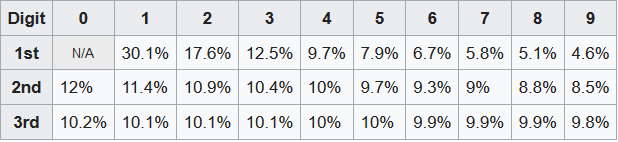
\includegraphics[scale=1]{wiki.jpg}
\end{figure}
\subsection{Drawbacks of Pinkham}
Hill state that the approach of Pinkham still have three drawbacks[Zhan3]. One is that the way he.  The set stated by him does not   have a  \emph{natural density}.
Natural density is the way we descrbie the prosibility to get one kind of number from a large set. Let A be a set of postive integers, then the natural density for A in the postive integers is defined as 
$$d(A)=\lim_{n\to \infty}\frac{A\cap\{1,2,3,...n\}}{n}$$
We can see that the set of positve even number have the natural density $\frac12$, but for the sets of postive integers $F_d$ whose first significant number is d, do not have the above property. [Zhan1]For example, if we let n=$10^k-1$, the
\begin{equation*}
\begin{aligned}
d(F_1)&=\lim_{n\to \infty}\frac{F_1\cap\{1,2,3,...n\}}{n}\\
&=\lim_{k\to \infty}\frac{\frac19(10^k-1)}{10^k-1}\\
&=\frac19
\end{aligned}
\end{equation*}
however, when n=$2*10^k-1$
\begin{equation*}
\begin{aligned}
d(F_1)&=\lim_{n\to \infty}\frac{F_1\cap\{1,2,3,...n\}}{n}\\
&=\lim_{k\to \infty}\frac{\frac19(10^k-1)+10^k}{2*10^k-1}\\
&=\lim_{k\to \infty}\frac{\frac{10}9*10^k}{2*10^k}\\
&=\frac59
\end{aligned}
\end{equation*}
So we can see the limit does not exist, which means the sets of postive integers $F_d$ whose first significant number is d, do not have natural density. 

Secondly, Pinkham's proof does not include the continous data and only focus on the infinite set inside of countable set. 

here would be more specific
% However, as Knuth pointed out (cf. Raimi [11]), there is no scale-invariant probabil ity measure on the Borel subsets of St+, since then the measure of the set (0, 1) must be the same as the measure of every interval (0, b), which by countable additivity must be 0.
\subsection{Hill's Proof}
\subsubsection{Drawbacks of Pinkham}
Hill states that the approach of Pinkham still have three drawbacks[Zhan3]. One is that the way he.  The set stated by him does not  have a  \emph{natural density}.

Natural density is the way we describe the possibility to get one kind of number from a large set. Let A be a set of positive integers, then the natural density for A in the positive integers is defined as 
$$d(A)=\lim_{n\to \infty}\frac{A\cap\{1,2,3,...n\}}{n}$$

We can see that the set of positve even number have the natural density $\frac12$, but for the sets of postive integers $F_d$ whose first significant number is d, do not have the above property. [Zhan1]For example, if we let n=$10^k-1$, the
\begin{equation*}
\begin{aligned}
d(F_1)&=\lim_{n\to \infty}\frac{F_1\cap\{1,2,3,...n\}}{n}\\
&=\lim_{k\to \infty}\frac{\frac19(10^k-1)}{10^k-1}\\
&=\frac19
\end{aligned}
\end{equation*}
however, when n=$2*10^k-1$
\begin{equation*}
\begin{aligned}
d(F_1)&=\lim_{n\to \infty}\frac{F_1\cap\{1,2,3,...n\}}{n}\\
&=\lim_{k\to \infty}\frac{\frac19(10^k-1)+10^k}{2*10^k-1}\\
&=\lim_{k\to \infty}\frac{\frac{10}9*10^k}{2*10^k}\\
&=\frac59
\end{aligned}
\end{equation*}

So we can see the limit does not exist, which means the sets of positive integers $F_d$ whose first significant number is d, do not have natural density. 

Secondly, Pinkham's proof does not include the continuous data. 


Lastly the previous proof focus on the finite sets inside of countable sets. 

here would be more specific
% However, as Knuth pointed out (cf. Raimi [11]), there is no scale-invariant probability measure on the Borel subsets of St+, since then the measure of the set (0, 1) must be the same as the measure of every interval (0, b), which by countable additivity must be 0.
\subsubsection{Mantissa Function}
\paragraph{Defination}
In the following,$\mathbb{Z}$ is the integers and $\mathbb{Z}^+$ is the postive integers,$\mathbb{B}$ is the Borel $\sigma$-algebra on $\mathbb{R}^+$, $\biguplus$ mean the union of disjoin sets. and for $E\subset\mathbb R$ and $a\in \mathbb R$, $aE=\{ae:e\in E\}$, $a+E=\{a+e:e\in E\}$



In order to solve the problems above and give a rigorous proof, Hill uses the \emph{mantissa function} M. For any integer b >1, the function $M_b$ is defined by 

$$M_b(x)=r, r\in [1,b), rb^n=x, n\in \mathbb{Z}$$

which is kind of like the \emph{division}, if we consider the x as the divisor, n as the quotient, and r is like the remainder. We can prove it is a well-defined function as following.

If it is not a well defined, then must exist x which make 
$$M_b(x)=r_1, M_b(x)=r_2,r_1\neq r_2$$ 
then by the difination, we can see that 
$$x=r_1*b^{n_1},x=r_2*b^{n_2}$$,
since $r_1\neq r_2$, we can get $n_1\neq n_2$, suppose $n_1 > n_2$, since $n_1,n_2 \in \mathbb{Z}$, so $n_1 \geq n_2+1$, so 
$$r_2=b^{n_1-n_2}*r_1\geq b*r_1$$
 however as $r_1\in [1,b)$, so $br_1\in [b,b^2)$ which is contradictory to $r_2\in [1,b)$.

\paragraph{mantissa $\sigma-$algebra}

Then consider its inverse function, we can see that it is not a well defined function as $M^{-1}(r)=\{x|x=rb^n,n\in\mathbb{Z}\}$. we can define an operation on the set. 


if $E\subset [1,b)$, then we define 
$$\langle E\rangle_b=M^{-1}_b\langle E\rangle=\biguplus_{n\in\mathbb Z} B^nE=\lbrace x|x=rb^n,r\in E, n\in \mathbb{Z}\rbrace$$

we extend use this to generate  the $\sigma$-algebra $\mathscr{M}_b$  by $M_b$, 
 $$\mathscr{M}_b=\{\langle E \rangle_b:E\in\mathbb{B}(1,b)\}$$

Hill shows $\mathscr{M}$ is closed under scalar multiplication.

If $S\in \mathscr{M}_b$, $a>0$ then as $\mathscr{M}_b=\{\langle E \rangle_b:E\in\mathbb{B}(1,b)\}$, we can see $S=\{\langle E_0\rangle_b\}$. Then we can find a new set $E_1$ which satisfy 
$$E_1=\{x'|x'=M_b(ax),x\in E_0\}$$
So $E_1$ also satisy $E_1\in\mathbb{B}(1,b)$ So $aS=\{\langle E_1\rangle_b\}\in \mathscr{M}_b$

Note here we can see if $S\in \mathscr{M}_b$,and $k\in\mathbb Z$, as $x=M_b{b^kx}$ for all x, so $10^kS=S$.
2.$\mathscr{M}_b\subset \mathscr{M}_{b^n}$ is self-similar.



\paragraph{Significant Digit}

we can define a function $D^{(i)}_{b}(x)$ which is the value of $i$th significant digit under tha base b, where b is an integer biger b> 1, and $i\in \mathbb{Z^{+}}$. For example,we can see that $D^{(1)}_b(x)=[M_b(x)]$ where [a] means the biggest integer that is smaller than a. In fact there is a connection between $M_b$ and $\{D_b^{i}\}$ which allows us to write $M_b$ by $\{D_b^{i}\}$

$$M_b(x)=\sum_{i=1}^{\infty}b^{1-i}D_b^{(i)}(x)$$

So for any postive interger b > 1 the $\sigma$-algebra $\mathscr{M}_b$ is generated by $M_b$, $\mathscr{M}_b$ can be generated by $\{D_b^{(i)} :i\in \mathbb{Z}^+\}$ . 


\subsubsection{General Significant-Digit Law}
Benford's law suggest that the probability for the first significant digit to be d equal
$$P( D^{(1)}_{10}=d)=log_{10}(1+d^{-1})$$
and the probability of the second significant digit to be d equal
$$P( D^{(2)}_{10}=d)=\sum^9_{k=1}log_{10}(1+(10k+d)^{-1})$$

Hill state that those two are just two special cases of the general significant-digit law, which is 

$$P(\bigcap^k_{i=1}\{D^{(i)}_b=d_i\})=log_b[1+(\sum^k_{i=1}B^{k-i}d_i)^{-1}]$$

Then he defines

$$\widehat P(E)=P(\langle E \rangle_b)$$

which build a connection between probabilty measures $P$ on $(R^+,\mathscr{M}_b)$ and the Borel probabilty measures $\widehat P$ on [1,b)

He proves the general significant-digit law base on the base-invariant.

\subsubsection{Base-invariant}



We call a probability measures $P$ on $(R^+,\mathscr{M}_b)$ is base-invariant when the corresponding Borel probability measures $\widehat P$ on [1,b) have the following property.

$$\widehat P[1,b^a)=\sum^{n-1}_{k=0}\widehat P[b^{k/n},b^{(k+a)/n})$$ 
for all $n\in \mathbb N$ and all $a\in (0,1)$

In order to prove this, we first prove a lemma, for $n\in \mathbb{Z}^+$
$$\langle E\rangle_b = \biguplus^{n-1}_{k=0}\langle b^kE\rangle_{b^n}$$
\begin{equation*}
\begin{aligned}
\langle E\rangle_b&=\lbrace x|x=rb^m,r\in E, m\in \mathbb{Z}\rbrace\\
&=\lbrace x|x=r*b^{km}*b^{nm},r\in E, n\in \mathbb{Z}^+,k\in{0...n}\rbrace\\
&=\biguplus^{n-1}_{k=0}\lbrace x|x=r*b^{nm},r\in E, n\in \mathbb{Z}\rbrace\\
&=\biguplus^{n-1}_{k=0}\langle b^kE\rangle_{b^n}
\end{aligned}
\end{equation*}

then as 
\begin{equation*}
\begin{aligned}
\widehat P[1,b^a)&=\widehat P(\langle E\rangle_b )\\
&=\widehat P(\biguplus^{n-1}_{k=0}\langle b^kE\rangle_{b^n})\\
&=\sum^{n-1}_{k=0}\widehat P(\langle b^kE\rangle_{b^n})\\
&=\sum^{n-1}_{k=0}\widehat P[b^{k/n},b^{(k+a)/n})
\end{aligned}
\end{equation*}
\subsubsection{Proof of Main Theorem}

First Hill proves a probability measure P on $(\mathbb{R}^+,\mathscr M_b)$ is \emph{base-invariant} if and only if for some q$\in [0,1]$,

$$P=qP_*+(1-q)P_b$$

where 
\begin{equation*}
\begin{aligned}
&P_*(\langle E\rangle_b)=\left\{
             \begin{array}{lr}
             1 &\text{if } 1\in E \\
             0 &\text{oherwise}
             \end{array}
\right.\\
&P_b(\langle [\alpha, \gamma \rangle_b)=\text{log}_b(\gamma/\alpha)
\end{aligned}
\end{equation*}

firstly we will prove if for some q$\in [0,1]$, P on $(\mathbb{R}^+,\mathscr M_b)$ satisfy $P=qP_*+(1-q)P_b$. 

$P_*$ is base-invariant, beacause  

\begin{equation*}
\begin{aligned}
&\widehat P_*[b^{k/n},b^{(k+a)/n})=\left\{
             \begin{array}{lr}
             1 &\text{if k=0 }  \\
             0 &\text{oherwise}
             \end{array}
\right.\\
&\widehat P_*[1,b^a)=1
\end{aligned}
\end{equation*}


and $P_b$ is also base invariant, because
\begin{equation*}
\begin{aligned}
\sum^{n-1}_{k=0}\widehat P_b[b^{k/n},b^{(k+a)/n})&=\sum^{n-1}_{k=0}\text{log}_bb^{\frac an}\\\
&=a\\
\widehat P_b[1,b^a)&=\text{log}_bb^a\\
&=a
\end{aligned}
\end{equation*}

So
\begin{equation*}
\begin{aligned}
\widehat P[1,b^a)&=q\widehat P_*[1,b^a)+(1-q)\widehat P_b[1,b^a)\\
&=q\sum^{n-1}_{k=0}\widehat P_*[b^{k/n},b^{(k+a)/n})+(1-q)\sum^{n-1}_{k=0}\widehat P_b[b^{k/n},b^{(k+a)/n})\\
&=\sum^{n-1}_{k=0}(q\widehat P_*[b^{k/n},b^{(k+a)/n})+(1-q)\widehat P_b[b^{k/n},b^{(k+a)/n}))\\
&=\sum^{n-1}_{k=0}\widehat P[b^{k/n},b^{(k+a)/n})\\
\end{aligned}
\end{equation*}


Next Hill prove if P on $(\mathbb{R}^+,\mathscr M_b)$ is base-invariant then  for some q$\in [0,1]$,

$$P=qP_*+(1-q)P_b$$

Let $\overline P$ be the b-logarithmic rescaling of $P$ on $\mathbb{B}[0,1)$ 
where $\overline P[0,a)=\widehat P[1,b^a)=P(\langle[1,b^a)\rangle_b)$ for all $a\in[0,1)$

\begin{equation*}
\begin{aligned}
\overline P[0,a) &=\widehat P[1,b^a)\\
&=\sum^{n-1}_{k=0}\widehat P[b^{k/n},b^{(k+a)/n})\\
&=\sum^{n-1}_{k=0}\overline P[\frac kn,\frac{(k+a)}n)
\end{aligned}
\end{equation*}

This suggest that $\overline P$ is \emph{invariant under the mapping} nx(mod 1) for all $n\in\mathbb{Z}^+$ which is if a measure $\mu$ on $(\Omega,\mathscr F)$ and for $T:\Omega \to \Omega$

$$\mu(E)=\mu(T^{-1}(E)) \text{for all }E\in F$$

Then we will prove a following lemma

If  A Borel probability measure $\overline P$ on [0,1) is \emph{invariant under the mapping} nx(mod 1) for all $n\in\mathbb{Z}^+$ then 

$$\overline P=q\delta_0+(1-q)\lambda \ \ \ \ \ n\in \mathbb Z$$
where $\lambda$ is Lebesgue measure on [0,1), and $\delta_0$ is the (Borel) Dirac (point s mass) measure at 0

Let $\phi_n,n\in\mathbb Z$ be the Fourier coefficients of $\overline P$

$$\phi_n=\int_0^1e^{2\pi*i*n*x}d\overline P(x),\ \ \ \ \ n\in\mathbb Z$$ as $\overline P$ on [0,1) is \emph{invariant under the mapping} nx(mod 1), let $\phi_n\equiv q$ for $\forall n\in \mathbb{Z}^+$where $q$ is real and in[0,1] while

$$\hat P({0})=\int_0^1\lim_{N\to \infty}e^{2\pi*i*n*x}d\overline P(x)=\lim_{N\to \infty}\frac1N\sum^N_{n=1}\phi_n=q$$


Then by the lemma, we can see that $\overline P_*$ is the $\delta_0$ which is  the (Borel) Dirac (point s mass) measure at 0 and $\overline P_b$ would be the $\lambda$ which is Lebesgue measure on [0,1) then we get

$$P=qP_*+(1-q)P_b$$

which get the general significant-digit law from Base-invariant.
\section{Synopsis}
\section{Reference}
\begin{enumerate}[-]
\item Wikipedia. Elastic properties of the elements. 
\\ \url{https://
en.wikipedia.org/w/index.php?title=Elastic_properties_of_the_elements_(data_page)} Web. Accessed June 20th, 2018
\item Pinkham, Roger S. \emph{On the distribution of first significant digits}. Ann. Math. Statist., 32(4):1223-1230, 12 1961.\\ \url{https://projecteuclid.org/euclid.aoms/1177704862}.
\item Wikipedia. Benford's Law. 
\\ \url{https://en.wikipedia.org/wiki/Benford%27s_law}
\item Theodore P. Hill. \emph{Base-invariance implies Benford’s law.} Proc. Amer. Math. Soc., 123:887–895, 1995. 
\\ \url{http://www.ams.org/journals/proc/1995-123-03/S0002-9939-1995-1233974-8/}.
\item Kuipers, L.; Niederreiter, H. (2006) [1974]. \emph{Uniform Distribution of Sequences}. Dover Publications. ISBN 0-486-45019-8. 
\item Mo, Guoduan; Liu, Kaidi. 2003. \emph{Function Approximation Method}. Science Press. ISBN 7-030-10914-7
\item Ma, Shanshan. \emph{A question about the natural number's density.} Journal of Jiangsu Normal University (2012).
\item Hill, Theodore P. \emph{The Significant-Digit Phenomenon.} American Mathematical Month l102.4(1995):322-327.
\end{enumerate}
\end{document}